MapReduce is a (functional) programming model for processing large amounts of data over a distributed network of nodes. Probably the most known implementation of MapReduce is Hadoop \cite{Hadoop}. MapReduce works by splitting the input data up into several partitions. Each partition is then sent off to a different node in the network, which in turn applies the map function on the data partition. This is called the map phase. The result of the map operation is usually stored temporarily on disk. Once all the partitions have been processed by the nodes in the network, the reduce phase is started. The nodes all read a specific range of the output from the map phase, and then apply the reduce function on that data. The resulting data is sent to an output file. An overview is given in figure \ref{fig:mapreduce}.

\begin{figure}[htb]
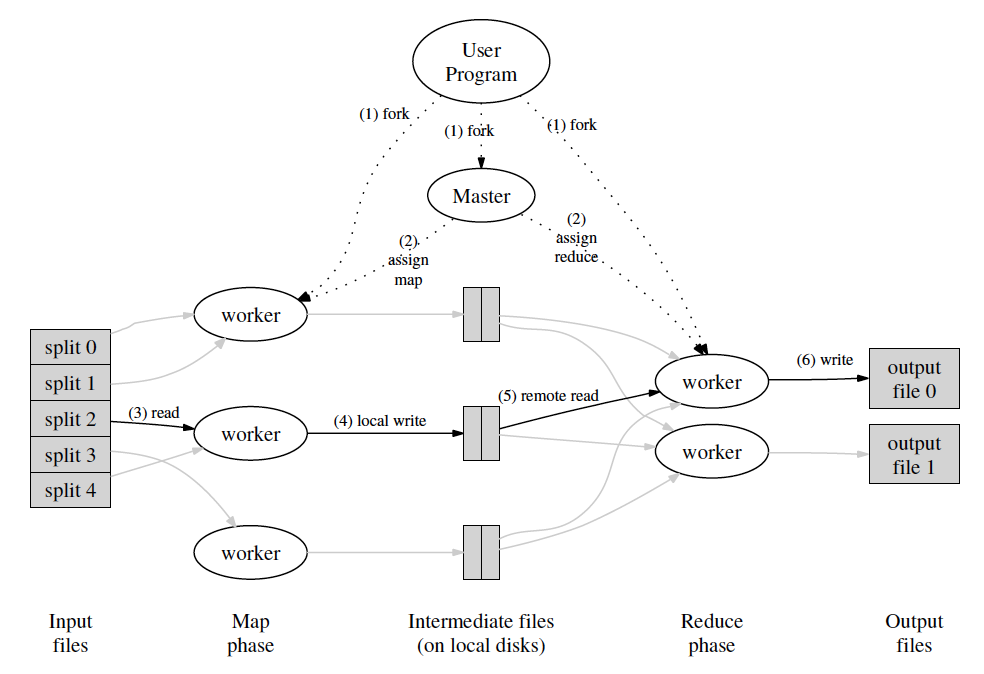
\includegraphics[width=340px]{mapreduce.png}
\caption{Image from: MapReduce: Simplified Data Processing on Large Clusters, 2004, by Jeffrey Dean and Sanjay Ghemawat}
\label{fig:mapreduce}
\end{figure}
